\chapter{Theoretical Background}
In this chapter we give a introduction in various topics and areas which are necessary in order to understand the implementation of our pipeline and how its generated results were computed. 

\section{Optical Flow}
\label{sec:optical_flow}
The optical flow is a visual phenomenon that describes the perception of motion.
By definition, it is the apparent visual motion a moving viewer experiences. To To give the reader a better, more intuitive understanding of this concept, have a look at figure $\ref{fig:motion_eg}$.
\begin{figure}[H]
\begin{center}
\subfigure[1st Frame]{
   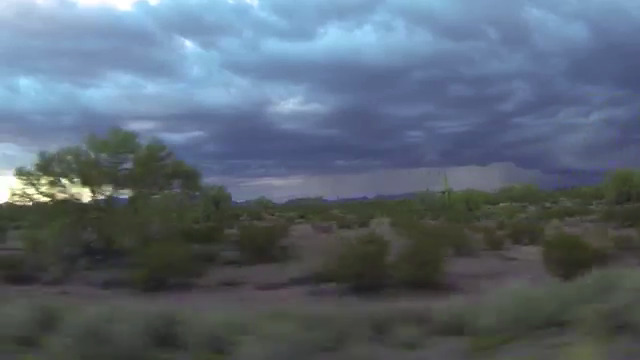
\includegraphics[width=0.47\linewidth] {background/of/ls1}
   \label{fig:motion_eg_f1}
}
\subfigure[2nd Frame]{
   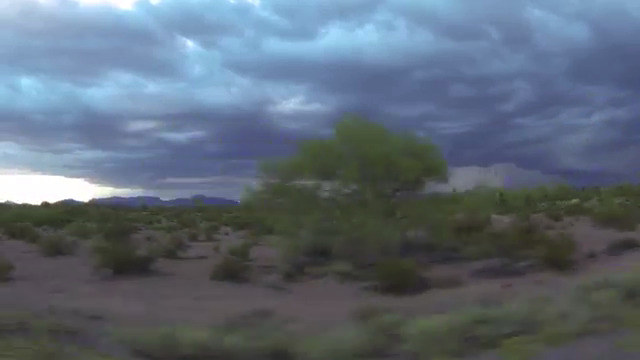
\includegraphics[width=0.47\linewidth] {background/of/ls2}
   \label{fig:motion_eg_f2}
}
~
\subfigure[3rd Frame]{
   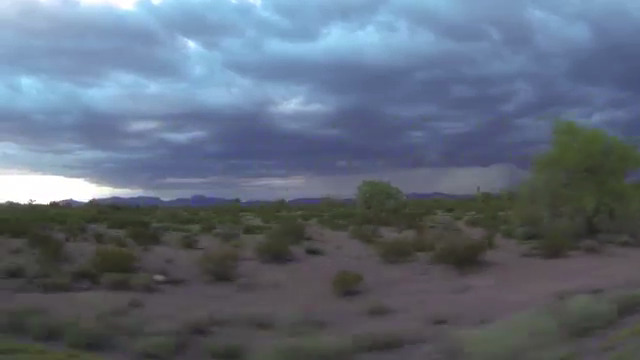
\includegraphics[width=0.47\linewidth] {background/of/ls3}
   \label{fig:motion_eg_f3}
}
\subfigure[4th Frame]{
   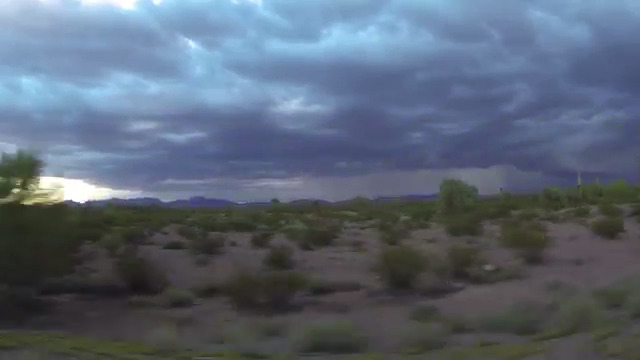
\includegraphics[width=0.47\linewidth] {background/of/ls4}
   \label{fig:motion_eg_f4}
}
\end{center}
\caption[Motion Example]{An example$\footnotemark$ of motion effects illustrated by four frames of a video sequence. Objects far away in the background, such as the mountain or the clouds seems to stand still. Objects being a fair distant apart, but also not too far away can be seen over several frames, such as the tree, that is passed. In addition, we also see observe, that the tree moves along the opposite direction as the driving car. Last, we also see the effect of motion blur for objects that are very close such as the grass.}
\label{fig:motion_eg}
\end{figure}
\footnotetext{The shown frames have been extracted from the following youtube video: \\ \url{https://www.youtube.com/watch?v=lo-pWLmMagc}}
Imagine you sit in a moving car and you are looking out of its windows. While doing so, you will observe that every overtaken object appear to move backwards. Furthermore, objects far in the background seem to stand still, whereas object close to the train seem to move very fast and thus have a blurry look. Therefore, the optical flow is an indicator for distance and size of an object. Moreover, the angle between the observer's viewing direction and the direction of the moving influences the optical flow. if an object travels perpendicular to the train or is directly above or below the it, then the optical flow is maximal. Lastly, an objects directly in front of a viewer will not exhibit any optical flow and thus appear to stand still. However, since not the whole object silhouette is directly in front of the viewer, its edges appear to move and therefore, the such an object appears to get either get larger or smaller, depending on its moving direction.

In summary, the optical flow has the following key properties:
\begin{itemize}
  \item Overtaken objects appear to move backwards.
  \item Distant objects seem to move very slowly and close objects appear to move fast.
  \item The magnitude of the optical flow is doubles if either the speed of the traveling viewer is doubled or the distance to the observed object is halved.
  \item The optical flow varies depending on the angle between the viewing direction and and the direction of movement of the observed object.
  \item The optical flow is maximal if either the object is moving orthogonally towards the viewer's direction or it is moving directly above or below it.
  \item Objects directly in front of a viewer exhibit no optical flow.
\end{itemize}

The underlying basis input of our whole approach depicts the optical flow, computed from a given inputs sequence.

%TODO: Write mathematical definition of the optical flow
The optical flow is a vector field that defines a point-to-point correspondence between two successive frames. Each vector acts as the displacement of a point in the first frame to match its corresponding point in the second frame.



\subsection{Determining Optical Flow - Berthold K.P. Horn and Brian G. Schnunck}
\label{sec:hs_formulation}

Is the distribution of apparent velocities of movement of brightness patterns in an image.
Can arise from relative motion of objects and the viewer.
Can give information about the spatial arrangement of the viewed objects and the rate of change in that arrangement.
Discontinuities in the optical flow can help to perform segmentation tasks.

the optical flow cannot be computed a point in the image independently of neighboring points without introducing additional constraints

reason: the velocity field any image point has two components while its change in image brightness due to motion yields only one constraint.

their example: consider a patch of a pattern where brightness varies as a function of one image coordinate, but not the other. Movement of the pattern in one direction alters the brightness at a particular point, but motion in the other direction yields no change. Thus components of movement in the latter direction cannot be determined locally.

their problem statement:
they initially assume that 

1. the surface is flat to avoid brightness variations due to shading effects.
2. the incident illumination is uniform across the surface. Then, the brightness at a point in the image is proportional to the reflectance of the surface at the corresponding point on the object.
3. reflectance varies smoothly and has no spatial discontinuities. Having no discontinuities assures that the image brightness is differentiable.
4. Situations where objects occlude one another are excluded.

derive equation that relates the change in image brightness at a point to the motion of the brightness pattern.

point $p(x,y)$, time $t$, brightness at p in the image plane at t $E(x,y,t)$.
When the pattern moves, the brightness of a particular point in the pattern is constant. 
$\frac{d E}{dt} = 0 <=> \frac{\partial E}{\partial x} \frac{x}{dt} + \frac{\partial E}{\partial y} \frac{y}{dt} + \frac{\partial E}{\partial t} = 0 <=> E_{x} u + E_{y} v + E_{t} = 0$.

where $u = \frac{dx}{dt}$ and $v = \frac{dy}{dt}$. Hence, we have a single linear equation with two unknowns $u$ and $v$.

solution: introduce a smoothness constraint.


\section{Motion Segmentation}
motion segmentation aims at decomposing a video in moving objects and background by segmenting the objects that undergo different motion patterns.

In this section we describe a conceptual approach how the motion segmentation task using optical flows is commonly approached in literature. 

\subsection{Spectral Clustering}
\subsection{Graph Cut}

multi-label CRF on superpixels for class segmentation $\cite{Fulkerson2009}$

\subsection{Kernighan-Lin Heuristic}


$\cite{Ker70}$
